\documentclass[12pt,a4paper]{article}
\usepackage[utf8]{inputenc}
\usepackage{amsmath}
\usepackage{amsfonts}
\usepackage{amssymb}
\usepackage{graphicx}
\usepackage{booktabs}
\usepackage{natbib}
\usepackage{dcolumn}
\usepackage{setspace}
\usepackage{array}
\usepackage{pdflscape} %allows for rotating pages with wide tables
\newcolumntype{P}[1]{>{\raggedright\arraybackslash}p{#1}}
%\usepackage{tabulary}
\usepackage[T1]{fontenc}
\usepackage{lmodern}
\usepackage{multirow}
\usepackage{multicol}

%\usepackage{mathptmx} %times font
%\usepackage{tgtermes} %times font
\usepackage[protrusion=true,expansion=true]{microtype}
\usepackage[top=1in, bottom=1in, left=1in, right=1in]{geometry}
\usepackage{hyperref}
\usepackage{color,soul} %highlighting
\usepackage{caption}
\captionsetup[figure]{labelfont=bf}
\captionsetup[table]{labelfont=bf}

%\usepackage{endnotes}
%\usepackage[heads,nolists,tablesfirst]{endfloat} %places tables and figures at the end
%



\usepackage{epstopdf}

\title{\textbf{Housing Bubbles and \\Support for Governing Parties}}


\author{
Frederik Hjorth \and Martin V. Larsen}

%, \textt{fh@ifs.ku.dk}, (+45) 26 27 24 41 }  } 


\begin{document}

\maketitle

\begin{center}
\textsc{draft - please do not quote, cite, or circulate}
\end{center}

\begin{abstract}
\noindent The real estate bubble which jump-started the great recession is one of the largest economic shocks that modern western economies have experienced. However, we know little about whether and how this housing bubble, or house prices in general, shape voters electoral behavior. In this paper we zoom in on one country, Denmark, which had one of the largest housing bubbles in the world, and examine how this rapid expansion and contraction of real estate prices shaped support for governing parties across four parliamentary elections. To do this, we link detailed data on local house prices to election returns at the precinct level. Across a wide range of demanding specifications we find that the when house prices increase governing parties get a higher vote share. Further, this relationship seems to be stronger in areas where house prices are very volatile, and when the change in house prices decrease. The findings hold important implications for the role of local economic conditions in voting behavior and for the political incentives faced by policy-makers.
 
\end{abstract}

%\begin{keyword}
%\doublespacing
%%x \sep y
%\end{keyword}

%\end{frontmatter}

\newpage

\onehalfspacing
%\doublespacing

\section{Introduction}

This is a study about how local economy shapes. Specifically, house prices.

Several possible mechanisms: punish/reward, updating estimates of competence; updating estimates of national economy.

Contributions to extant research.
\begin{itemize}
	\item Data: Small geographical units + multiple elections + population based data-
	\item House prices: Almost never done - although Lenz and Healy sort of similar.
	\item Empirical setting: Big bubble - Denmark (both pro and con - possibly least likely cf. general low economic voting)
\end{itemize}

These different factors make causal identification more likely in this study, than it has been before. 

Add to this by also exploring negativity bias - especially important given the "bubblyness" of house prices. If voters respond uniformly or not this will present governments with widely different incentives. 



\section{Empirical Setting}

Denmark's housing market.

Denmark's political situation.
Peter Birch!


\section{Data}

How did we get data in IV and DV

\section{Results}

\begin{table}[htbp]\centering
\def\sym#1{\ifmmode^{#1}\else\(^{#1}\)\fi}
\caption{Estimated effects of house prices on electoral support for governing parties.} \label{tab1}
\begin{tabular}{l*{5}{c}}
\hline\hline
                    &\multicolumn{1}{c}{(1)}        &\multicolumn{1}{c}{(2)}        &\multicolumn{1}{c}{(3)}        &\multicolumn{1}{c}{(4)}        &\multicolumn{1}{c}{(5)}        \\
\hline
$\Delta$ house price&        0.10\sym{**}&        0.12\sym{**}&        0.05\sym{**}&        0.05\sym{**}&        0.01\sym{*} \\
                    &      (0.01)        &      (0.01)        &      (0.01)        &      (0.01)        &      (0.01)        \\
[1em]
\hline Precinct FE  &                    &$\checkmark$        &$\checkmark$        &$\checkmark$        &$\checkmark$        \\
[1em]
Year FE             &                    &                    &$\checkmark$        &$\checkmark$        &$\checkmark$        \\
[1em]
Year FE * Structural factors&                    &                    &                    &$\checkmark$        &$\checkmark$        \\
[1em]
Year FE * Municipality FE&                    &                    &                    &                    &$\checkmark$        \\
\hline
Observations        &        4192        &        4192        &        4192        &        4170        &        4170        \\
RMSE                &        8.40        &        7.16        &        5.71        &        4.77        &        2.84        \\
\hline\hline
\multicolumn{6}{l}{\footnotesize Standard errors in parentheses}\\
\multicolumn{6}{l}{\footnotesize \sym{*} \(p<0.05\), \sym{**} \(p<0.01\)}\\
\end{tabular}
\end{table}


\subsection{Causal identification}

\begin{table}[htbp]\centering
\def\sym#1{\ifmmode^{#1}\else\(^{#1}\)\fi}
\caption{Estimated effects of house prices on electoral support for governing parties at t+1.} \label{tab2}
\begin{tabular}{l*{5}{c}}
\hline\hline
                    &\multicolumn{1}{c}{(1)}        &\multicolumn{1}{c}{(2)}        &\multicolumn{1}{c}{(3)}        &\multicolumn{1}{c}{(4)}        &\multicolumn{1}{c}{(5)}        \\
\hline
$\Delta$ house price&        0.12\sym{**}&        0.14\sym{**}&       -0.02        &       -0.01        &        0.02        \\
                    &      (0.01)        &      (0.01)        &      (0.01)        &      (0.01)        &      (0.01)        \\
[1em]
\hline Precinct FE  &                    &$\checkmark$        &$\checkmark$        &$\checkmark$        &$\checkmark$        \\
[1em]
Year FE             &                    &                    &$\checkmark$        &$\checkmark$        &$\checkmark$        \\
[1em]
Year FE * Structural factors&                    &                    &                    &$\checkmark$        &$\checkmark$        \\
[1em]
Year FE * Municiplaity FE&                    &                    &                    &                    &$\checkmark$        \\
\hline
Observations        &        3227        &        3227        &        3227        &        3209        &        3209        \\
RMSE                &        8.62        &        7.11        &        6.22        &        5.24        &        3.05        \\
\hline\hline
\multicolumn{6}{l}{\footnotesize Standard errors in parentheses}\\
\multicolumn{6}{l}{\footnotesize \sym{*} \(p<0.05\), \sym{**} \(p<0.01\)}\\
\end{tabular}
\end{table}


\begin{table}[htbp]\centering
\def\sym#1{\ifmmode^{#1}\else\(^{#1}\)\fi}
\caption{Estimated effects of house prices on electoral support for governing parties at t-1.} \label{tab3}
\begin{tabular}{l*{4}{c}}
\hline\hline
                    &\multicolumn{1}{c}{(1)}        &\multicolumn{1}{c}{(2)}        &\multicolumn{1}{c}{(3)}        &\multicolumn{1}{c}{(4)}        \\
\hline
$\Delta$ house price&       -0.03\sym{**}&       -0.04\sym{**}&        0.07\sym{**}&        0.08\sym{**}\\
                    &      (0.01)        &      (0.01)        &      (0.01)        &      (0.01)        \\
[1em]
\hline Precinct FE  &                    &$\checkmark$        &$\checkmark$        &$\checkmark$        \\
[1em]
Year FE             &                    &                    &$\checkmark$        &$\checkmark$        \\
[1em]
Year FE * Structural factors&                    &                    &                    &$\checkmark$        \\
\hline
Observations        &        4197        &        4197        &        4197        &        4173        \\
RMSE                &        8.80        &        7.50        &        6.46        &        5.04        \\
\hline\hline
\multicolumn{5}{l}{\footnotesize Standard errors in parentheses}\\
\multicolumn{5}{l}{\footnotesize \sym{*} \(p<0.05\), \sym{**} \(p<0.01\)}\\
\end{tabular}
\end{table}


\subsection{Evidence of a grievance asymmetry}

\begin{table}[htbp]\centering
\def\sym#1{\ifmmode^{#1}\else\(^{#1}\)\fi}
\caption{Estimated effects of house prices on electoral support for governing parties across positive and negative changes.} \label{tab4}
\begin{tabular}{l*{4}{c}}
\hline\hline
                    &\multicolumn{1}{c}{(1)}         &\multicolumn{1}{c}{(2)}         &\multicolumn{1}{c}{(3)}         &\multicolumn{1}{c}{(4)}         \\
\hline
$\Delta$ house price (negative)&       -0.08\sym{***}&       -0.11\sym{***}&       -0.07\sym{***}&       -0.10\sym{***}\\
                    &      (0.02)         &      (0.03)         &      (0.02)         &      (0.02)         \\
[1em]
$\Delta$ house price (positive)&        0.12\sym{***}&        0.12\sym{***}&        0.04\sym{***}&        0.04\sym{**} \\
                    &      (0.01)         &      (0.02)         &      (0.01)         &      (0.01)         \\
[1em]
\hline Precinct  FE &                     &$\checkmark$         &$\checkmark$         &$\checkmark$         \\
[1em]
Year FE             &                     &                     &$\checkmark$         &$\checkmark$         \\
[1em]
Year FE * Structural factors&                     &                     &                     &$\checkmark$         \\
\hline
Test of no difference (p)&        0.26         &        0.84         &        0.24         &        0.02         \\
Observations        &        4192         &        4192         &        4192         &        4170         \\
RMSE                &        8.41         &        7.16         &        5.71         &        4.77         \\
\hline\hline
\multicolumn{5}{l}{\footnotesize Standard errors in parentheses}\\
\multicolumn{5}{l}{\footnotesize \sym{*} \(p<0.05\), \sym{**} \(p<0.01\), \sym{***} \(p<0.001\)}\\
\end{tabular}
\end{table}


\subsection{Evidence of a  bubblyness-effect}

\begin{table}[htbp]\centering
\def\sym#1{\ifmmode^{#1}\else\(^{#1}\)\fi}
\caption{Estimated effects of house prices on electoral support for governing parties across volatility.} \label{tab5}
\begin{tabular}{l*{4}{c}}
\hline\hline
                    &\multicolumn{1}{c}{(1)}        &\multicolumn{1}{c}{(2)}        &\multicolumn{1}{c}{(3)}        &\multicolumn{1}{c}{(4)}        \\
\hline
$\Delta$ housing price&       -0.01        &       -0.20\sym{**}&       -0.18\sym{**}&       -0.17\sym{**}\\
                    &      (0.03)        &      (0.02)        &      (0.02)        &      (0.03)        \\
[1em]
Log(density)        &       -5.49\sym{**}&       -2.69\sym{**}&        0.00        &        0.00        \\
                    &      (0.37)        &      (0.41)        &         (.)        &         (.)        \\
[1em]
$\Delta$ housing price $\times$ Log(density)&        0.05\sym{**}&        0.12\sym{**}&        0.10\sym{**}&        0.10\sym{**}\\
                    &      (0.01)        &      (0.01)        &      (0.01)        &      (0.01)        \\
[1em]
\hline Precinct FE  &                    &                    &$\checkmark$        &$\checkmark$        \\
[1em]
Year FE             &                    &                    &                    &$\checkmark$        \\
\hline
Observations        &        4193        &        4173        &        4173        &        4173        \\
RMSE                &        8.42        &        6.80        &        5.50        &        5.40        \\
\hline\hline
\multicolumn{5}{l}{\footnotesize Standard errors in parentheses}\\
\multicolumn{5}{l}{\footnotesize \sym{*} \(p<0.05\), \sym{**} \(p<0.01\)}\\
\end{tabular}
\end{table}


\begin{figure}
	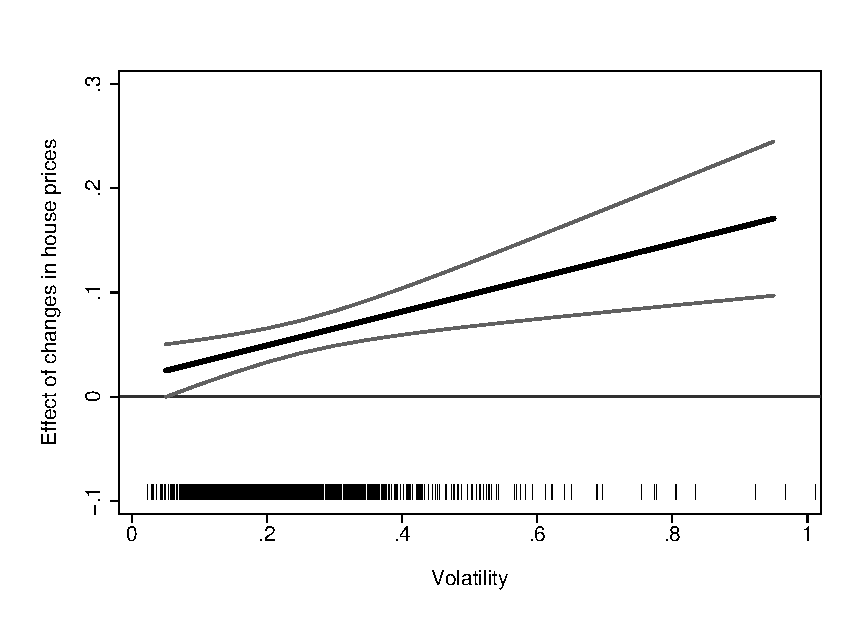
\includegraphics[width=0.8\textwidth]{../figures/volatilityinteraction.eps}
	\centering
	\caption{Marginal effect of $\Delta$house prices on incumbent support across levels of price volatility with 95 pct. Confidence Intervals. Rug plot signifies distribution of observations across the volatility variable.}
\end{figure}

\begin{table}[htbp]\centering
\def\sym#1{\ifmmode^{#1}\else\(^{#1}\)\fi}
\caption{Estimated effects of house prices on electoral support for governing parties across volatility.} \label{tab6}
\begin{tabular}{l*{5}{c}}
\hline\hline
                    &\multicolumn{1}{c}{(1)}        &\multicolumn{1}{c}{(2)}        &\multicolumn{1}{c}{(3)}        &\multicolumn{1}{c}{(4)}        &\multicolumn{1}{c}{(5)}        \\
\hline
$\Delta$ house price (positive)&        0.15\sym{**}&        0.11\sym{**}&        0.02        &        0.03        &       -0.04\sym{*} \\
                    &      (0.03)        &      (0.04)        &      (0.03)        &      (0.02)        &      (0.02)        \\
[1em]
$\Delta$ house price (negative)&       -0.05        &       -0.16\sym{*} &        0.03        &        0.02        &       -0.07\sym{*} \\
                    &      (0.07)        &      (0.06)        &      (0.05)        &      (0.05)        &      (0.03)        \\
[1em]
Volatility          &       -7.22        &        0.14        &        7.29\sym{**}&       -1.16        &       -1.73        \\
                    &      (3.72)        &      (3.25)        &      (2.70)        &      (2.03)        &      (1.60)        \\
[1em]
$\Delta$ house price (positive) $\times$ Volatility&       -0.10        &        0.04        &        0.05        &        0.03        &        0.19\sym{**}\\
                    &      (0.12)        &      (0.13)        &      (0.09)        &      (0.07)        &      (0.06)        \\
[1em]
$\Delta$ house price (negative) $\times$ Volatility&       -0.01        &        0.19        &       -0.54\sym{**}&       -0.50\sym{**}&        0.12        \\
                    &      (0.28)        &      (0.24)        &      (0.21)        &      (0.17)        &      (0.12)        \\
[1em]
\hline Precinct FE  &                    &$\checkmark$        &$\checkmark$        &$\checkmark$        &$\checkmark$        \\
[1em]
Year FE             &                    &                    &$\checkmark$        &$\checkmark$        &$\checkmark$        \\
[1em]
Year FE * Structural factors&                    &                    &                    &$\checkmark$        &$\checkmark$        \\
[1em]
Year FE * Municipality FE&                    &                    &                    &                    &$\checkmark$        \\
\hline
Observations        &        4184        &        4184        &        4184        &        4162        &        4162        \\
RMSE                &        8.46        &        7.17        &        5.70        &        4.76        &        2.84        \\
\hline\hline
\multicolumn{6}{l}{\footnotesize Standard errors in parentheses}\\
\multicolumn{6}{l}{\footnotesize \sym{*} \(p<0.05\), \sym{**} \(p<0.01\)}\\
\end{tabular}
\end{table}





\section{Discussion}

How causally convincing is our results?

Is the negativity bias really a bias? Maybe... maybe not.

Implications for policy makers.

Goodnight!



%Appendikser
%Overvej et om forhold mellem volatilitet og prisændringer
%Overvej et på et andet kontekstuelt niveau - e.g. kommuner - jf. MAUP.
%Overvej et om robusthed af interaktionsled - evt. lav kommuneinteraktioner, og se om effekten stadig holder
%Overvej det samme som sidste om positiv-negativ





\clearpage

\singlespacing

\bibliographystyle{../../bibliography/model2-names}
\bibliography{../../bibliography/library}

\end{document}
